\documentclass[../main.tex]{subfiles}

\begin{document}
Trong chương này, đồ án tập trung xác định yêu cầu, phân tích và thiết kế các 
chức năng của hệ thống.

\section{Xác định yêu cầu hệ thống}
\label{sec:2.1}

\subsection{Xác định các Actor}
\label{sec:2.1.1}
Hệ thống gồm 2 tác nhân chính: \textbf{Người dùng (User)}, \textbf{Quản trị viên (Admin)}.

\begin{table}[H]
    \centering
    \caption{Danh sách các Actor}
    \label{tab:ch3_actors}
    \begin{tabular}{|>{\centering\arraybackslash}p{0.08\textwidth}|>{\raggedright\arraybackslash}p{0.18\textwidth}|>{\raggedright\arraybackslash}p{0.60\textwidth}|}
        \hline
        \multicolumn{1}{|c|}{\textbf{STT}} & \multicolumn{1}{c|}{\textbf{Actor}} & \multicolumn{1}{c|}{\textbf{Mô tả}} \\
        \hline
        1 & Admin & Là quản trị viên hệ thống có thể thực hiện các nghiệp vụ quản lý như: quản lý dữ liệu về món ăn, bệnh, người dùng và xem thống kê hệ thống. \\
        \hline
        2 & User & Là người dùng cuối, có thể nhận diện món ăn bằng hình ảnh, tìm kiếm, xem chi tiết món ăn, lưu, xem lịch sử bữa ăn, so sánh món ăn, lập kế hoạch bữa ăn, quản lý công thức món ăn cá nhân và xem thống kê. \\
        \hline
    \end{tabular}
\end{table}

\subsection{Xác định các UseCase}
\label{sec:2.1.2}

\begin{longtable}{|>{\centering\arraybackslash}p{0.06\textwidth}|>{\raggedright\arraybackslash}p{0.24\textwidth}|>{\raggedright\arraybackslash}p{0.17\textwidth}|>{\raggedright\arraybackslash}p{0.39\textwidth}|}
    \caption{Danh sách các UseCase trong hệ thống}
    \label{tab:ch2_usecases} \\
    \hline
    \multicolumn{1}{|c|}{\textbf{STT}} & \multicolumn{1}{c|}{\textbf{UseCase}} & \multicolumn{1}{c|}{\textbf{Actor}} & \multicolumn{1}{c|}{\textbf{Mục đích chính}} \\
    \hline
    \endfirsthead
    \hline
    \multicolumn{1}{|c|}{\textbf{STT}} & \multicolumn{1}{c|}{\textbf{UseCase}} & \multicolumn{1}{c|}{\textbf{Actor}} & \multicolumn{1}{c|}{\textbf{Mục đích chính}} \\
    \hline
    \endhead
    \hline
    \endfoot
    1 & \textbf{Đăng ký tài khoản} & Người dùng & Tạo tài khoản mới bằng Email và mật khẩu để sử dụng hệ thống. \\
    \hline
    2 & \textbf{Đăng nhập bằng Email/Mật khẩu} & Người dùng & Xác thực tài khoản người dùng qua Email và mật khẩu để truy cập ứng dụng. \\
    \hline
    3 & \textbf{Đăng nhập bằng Google} & Người dùng & Đăng nhập nhanh vào hệ thống thông qua tài khoản Google (OAuth2). \\
    \hline
    4 & \textbf{Quên mật khẩu} & Người dùng & Khôi phục hoặc đặt lại mật khẩu khi người dùng không nhớ mật khẩu đăng nhập. \\
    \hline
    5 & \textbf{Đổi mật khẩu} & Người dùng & Cập nhật mật khẩu mới nhằm đảm bảo an toàn cho tài khoản cá nhân. \\
    \hline
    6 & \textbf{Đăng xuất} & Người dùng & Kết thúc phiên làm việc hiện tại và thoát khỏi tài khoản trên thiết bị. \\
    \hline
    7 & \textbf{Quản lý hồ sơ sức khỏe} & Người dùng & Tạo và cập nhật thông tin thể trạng (chiều cao, cân nặng, dị ứng, mục tiêu) để tính chỉ số BMI, TDEE. \\
    \hline
    8 & \textbf{Ghi nhật ký bữa ăn} & Người dùng & Lưu lại các bữa ăn hằng ngày (thủ công, nhận diện ảnh AI hoặc quét mã vạch) để theo dõi calo và dinh dưỡng. \\
    \hline
    9 & \textbf{Quản lý món ăn tùy chỉnh} & Người dùng & Thêm, chỉnh sửa hoặc xóa các món ăn và công thức cá nhân do người dùng tự tạo. \\
    \hline
    10 & \textbf{Xem gợi ý thực đơn cá nhân hóa} & Người dùng & Xem thực đơn được AI đề xuất dựa trên mục tiêu calo, dị ứng và ngân sách. \\
    \hline
    11 & \textbf{Trò chuyện với Chatbot dinh dưỡng} & Người dùng & Hỏi đáp, nhận tư vấn về chế độ ăn uống và dinh dưỡng từ Chatbot AI. \\
    \hline
    12 & \textbf{Ghi nhật ký tập luyện} & Người dùng & Lưu lại các hoạt động thể chất, thời gian tập và lượng calo tiêu thụ. \\
    \hline
    13 & \textbf{Đồng bộ dữ liệu với Google Fit} & Người dùng & Tự động đồng bộ số bước chân, nhịp tim và dữ liệu vận động từ Google Fit. \\
    \hline
    14 & \textbf{Xem lịch sử cân nặng} & Người dùng & Theo dõi biểu đồ và lịch sử biến động cân nặng theo thời gian. \\
    \hline
    15 & \textbf{Ghi nhận cân nặng} & Người dùng & Cập nhật chỉ số cân nặng hiện tại vào hệ thống theo dõi sức khỏe. \\
    \hline
    16 & \textbf{Ghi nhận lượng nước uống} & Người dùng & Lưu lại lượng nước đã uống trong ngày để đảm bảo mục tiêu cấp nước. \\
    \hline
    17 & \textbf{Xem tổng quan Dashboard} & Người dùng & Theo dõi nhanh tiến độ calo, macro, lượng nước, bước chân và chuỗi streak trong ngày. \\
    \hline
    18 & \textbf{Xem chuỗi ngày mục tiêu} & Người dùng & Kiểm tra số ngày liên tiếp đạt mục tiêu dinh dưỡng và vận động. \\
    \hline
    19 & \textbf{Tham gia thử thách} & Người dùng & Đăng ký tham gia các thử thách sức khỏe để tăng động lực rèn luyện. \\
    \hline
    20 & \textbf{Xem huy hiệu} & Người dùng & Xem danh sách các huy hiệu và thành tích đã đạt được trong quá trình sử dụng. \\
    \hline
    21 & \textbf{Quản lý bạn bè} & Người dùng & Tìm kiếm, kết bạn và quản lý danh sách bạn bè trong hệ thống. \\
    \hline
    22 & \textbf{Xem bảng xếp hạng} & Người dùng & Xem thứ hạng thành tích và điểm số của bản thân so với bạn bè. \\
    \hline
    23 & \textbf{Đăng nhập} & Quản trị viên & Xác thực tài khoản quản trị để truy cập vào hệ thống quản lý. \\
    \hline
    24 & \textbf{Quản lý người dùng} & Quản trị viên & Xem danh sách, phân quyền, khóa hoặc mở khóa tài khoản người dùng. \\
    \hline
    25 & \textbf{Quản lý món ăn} & Quản trị viên & Thêm, sửa, xóa và cập nhật thông tin dinh dưỡng của các món ăn trong hệ thống. \\
    \hline
    26 & \textbf{Quản lý nguyên liệu} & Quản trị viên & Quản lý danh mục nguyên liệu và giá trị dinh dưỡng cấu thành món ăn. \\
    \hline
    27 & \textbf{Quản lý loại hình vận động} & Quản trị viên & Thêm, sửa, xóa các loại bài tập và hệ số tiêu thụ calo tương ứng. \\
    \hline
    28 & \textbf{Quản lý bệnh lý nền} & Quản trị viên & Quản lý danh sách các bệnh mãn tính và các lưu ý, kiêng kỵ dinh dưỡng liên quan. \\
    \hline
    29 & \textbf{Quản lý huy hiệu} & Quản trị viên & Tạo mới, chỉnh sửa điều kiện đạt được và quản lý các huy hiệu trong hệ thống. \\
    \hline
    30 & \textbf{Quản lý thử thách} & Quản trị viên & Thiết lập, cập nhật và quản lý các thử thách sức khỏe dành cho người dùng. \\
    \hline
    31 & \textbf{Quản lý thông báo} & Quản trị viên & Tạo, gửi và quản lý các thông báo hệ thống tới người dùng. \\
    \hline
    32 & \textbf{Xem Dashboard \& Thống kê} & Quản trị viên & Theo dõi các chỉ số tổng quan, lượng người dùng hoạt động và thống kê toàn hệ thống. \\
    \hline
\end{longtable}

\section{Phân tích thiết kế hệ thống}
\label{sec:2.2}

\subsection{Biểu đồ UseCase tổng quát}
\label{sec:2.2.1}

\begin{figure}[H]
    \centering
    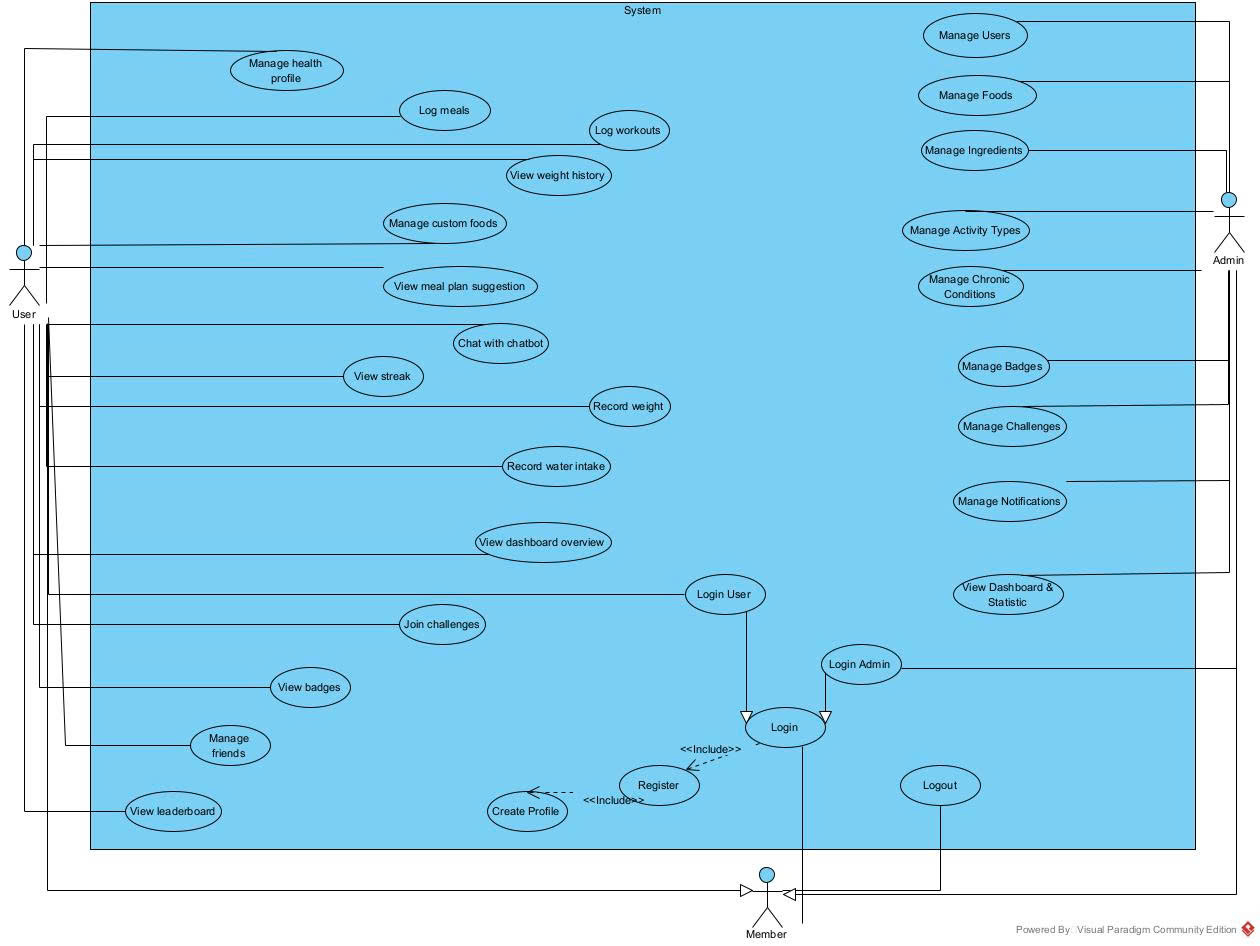
\includegraphics[width=\textwidth,height=0.85\textheight,keepaspectratio]{img/usecase_tong_quat.jpg}
    \caption{Biểu đồ UseCase tổng quát}
    \label{fig:usecase_tong_quan}
\end{figure}

\subsection{Phân rã biểu đồ UseCase}
\label{sec:2.2.2}

% \begin{figure}[H]
%     \centering
%     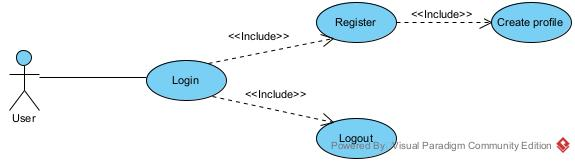
\includegraphics[width=0.85\textwidth]{img/usecase_register.jpg}
%     \caption{Biểu đồ UseCase chức năng đăng ký, đăng nhập và đăng xuất}
%     \label{fig:usecase_register}
% \end{figure}

\subsection{Kịch bản chuẩn và ngoại lệ}
\label{sec:2.2.3}

\subsection{Biểu đồ lớp thực thể}
\label{sec:2.2.4}

\begin{figure}[H]
    \centering
    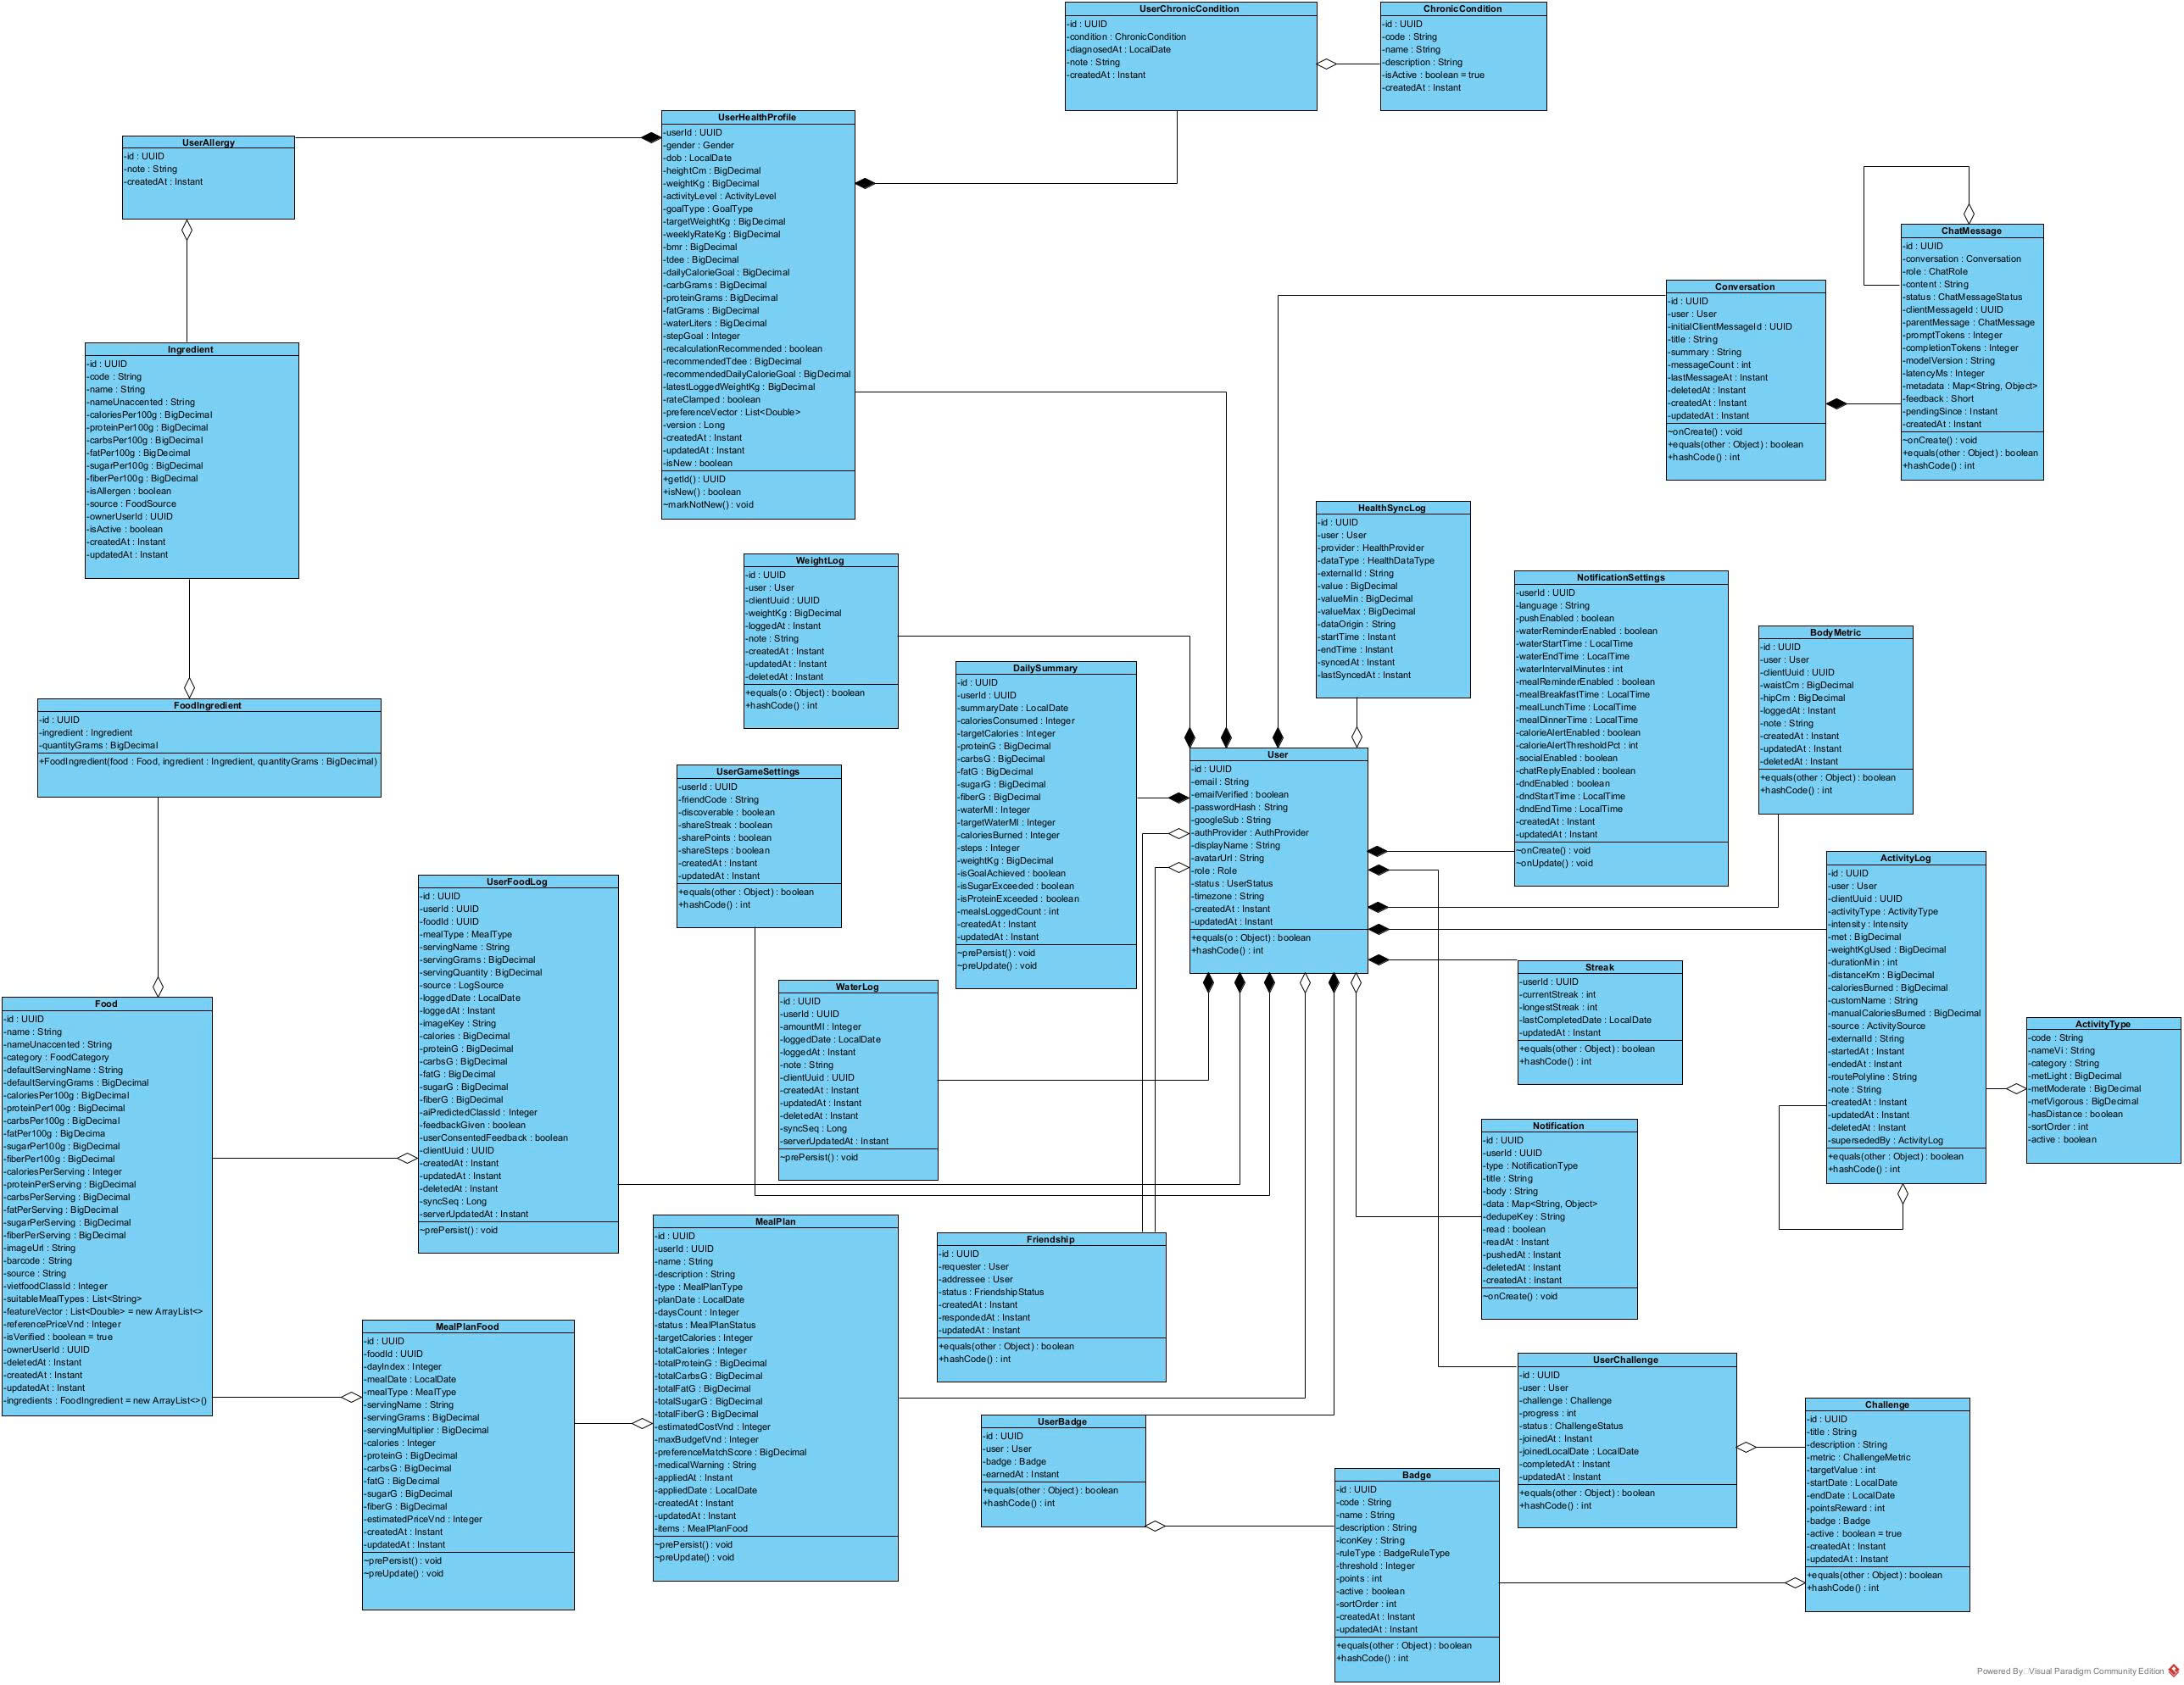
\includegraphics[width=\textwidth,height=0.85\textheight,keepaspectratio]{img/class_diagram.jpg}
    \caption{Biểu đồ lớp thực thể}
    \label{fig:class_diagram}
\end{figure}

\subsection{Biểu đồ trạng thái}
\label{sec:2.2.5}

\subsection{Sơ đồ tuần tự}
\label{sec:2.2.6}

\section{Thiết kế cơ sở dữ liệu}
\label{sec:2.3}

\subsection{Mô tả cấu trúc cơ sở dữ liệu}
\label{sec:2.3.1}

\begin{longtable}{|>{\centering\arraybackslash}p{0.07\textwidth}|>{\raggedright\arraybackslash}p{0.31\textwidth}|>{\raggedright\arraybackslash}p{0.50\textwidth}|}
    \caption{Mô tả cơ sở dữ liệu tổng quát}
    \label{tab:ch2_db_overview} \\
    \hline
    \multicolumn{1}{|c|}{\textbf{STT}} & \multicolumn{1}{c|}{\textbf{Tên bảng}} & \multicolumn{1}{c|}{\textbf{Mô tả}} \\
    \hline
    \endfirsthead
    \hline
    \multicolumn{1}{|c|}{\textbf{STT}} & \multicolumn{1}{c|}{\textbf{Tên bảng}} & \multicolumn{1}{c|}{\textbf{Mô tả}} \\
    \hline
    \endhead
    \hline
    \endfoot
    1 & users & Lưu trữ thông tin tài khoản đăng nhập, xác thực (Email/Google) và thông tin cá nhân người dùng. \\
    \hline
    2 & user\_health\_profiles & Lưu trữ hồ sơ sức khỏe, thể trạng, mục tiêu cân nặng và các chỉ số tính toán (BMI, TDEE, calo mục tiêu). \\
    \hline
    3 & chronic\_conditions & Danh mục các bệnh lý nền / mãn tính dùng cho cảnh báo và gợi ý dinh dưỡng. \\
    \hline
    4 & user\_chronic\_conditions & Liên kết người dùng với các bệnh lý nền đang mắc phải và ngày chẩn đoán. \\
    \hline
    5 & ingredients & Danh mục nguyên liệu thực phẩm kèm thông tin giá trị dinh dưỡng trên 100g. \\
    \hline
    6 & user\_allergies & Lưu trữ danh sách các nguyên liệu gây dị ứng của từng người dùng. \\
    \hline
    7 & foods & Danh mục món ăn (chuẩn và tùy chỉnh), giá trị dinh dưỡng, mã vạch và nhãn nhận diện AI. \\
    \hline
    8 & food\_ingredients & Bảng trung gian mô tả thành phần nguyên liệu và định lượng cấu thành từng món ăn. \\
    \hline
    9 & meal\_plans & Lưu trữ thông tin các kế hoạch thực đơn cá nhân hóa theo ngày và ngân sách. \\
    \hline
    10 & meal\_plan\_foods & Chi tiết danh sách các món ăn, khẩu phần và dinh dưỡng trong từng thực đơn. \\
    \hline
    11 & user\_food\_logs & Nhật ký ghi nhận các bữa ăn hằng ngày của người dùng (thủ công, ảnh AI hoặc mã vạch). \\
    \hline
    12 & activity\_types & Danh mục các loại hình vận động và hệ số tiêu thụ năng lượng (MET) theo cường độ. \\
    \hline
    13 & activity\_logs & Nhật ký ghi nhận các hoạt động tập luyện, thời gian và lượng calo tiêu thụ của người dùng. \\
    \hline
    14 & health\_sync\_logs & Lưu trữ dữ liệu sức khỏe đồng bộ từ thiết bị/nền tảng ngoài như Google Fit. \\
    \hline
    15 & weight\_logs & Lưu trữ lịch sử ghi nhận cân nặng theo thời gian của người dùng. \\
    \hline
    16 & body\_metrics & Lưu trữ các chỉ số đo cơ thể (vòng eo, vòng hông) theo thời gian. \\
    \hline
    17 & water\_logs & Nhật ký ghi nhận lượng nước uống hằng ngày của người dùng. \\
    \hline
    18 & daily\_summaries & Tổng hợp chỉ số dinh dưỡng, vận động, nước uống và tiến độ đạt mục tiêu theo ngày. \\
    \hline
    19 & streaks & Theo dõi chuỗi ngày liên tiếp đạt mục tiêu (streak hiện tại và dài nhất) của người dùng. \\
    \hline
    20 & badges & Danh mục các huy hiệu thành tích, điều kiện đạt được và điểm thưởng. \\
    \hline
    21 & user\_badges & Lưu trữ danh sách các huy hiệu mà người dùng đã đạt được. \\
    \hline
    22 & challenges & Danh mục các thử thách sức khỏe, chỉ tiêu, thời gian áp dụng và phần thưởng. \\
    \hline
    23 & user\_challenges & Lưu trữ thông tin tham gia và tiến độ hoàn thành thử thách của người dùng. \\
    \hline
    24 & friendships & Quản lý mối quan hệ kết bạn và trạng thái lời mời kết bạn giữa các người dùng. \\
    \hline
    25 & user\_game\_settings & Lưu trữ cấu hình riêng tư và hiển thị trong tính năng trò chơi hóa (bạn bè, bảng xếp hạng). \\
    \hline
    26 & notification\_settings & Lưu trữ tùy chọn nhận thông báo nhắc nhở (uống nước, bữa ăn, cảnh báo calo, DND). \\
    \hline
    27 & notifications & Lưu trữ lịch sử thông báo gửi đến người dùng và trạng thái đã đọc. \\
    \hline
    28 & conversations & Lưu trữ danh sách các phiên hội thoại giữa người dùng và Chatbot tư vấn dinh dưỡng AI. \\
    \hline
    29 & chat\_messages & Lưu trữ chi tiết nội dung tin nhắn, phản hồi và thông tin suy luận trong từng hội thoại. \\
    \hline
\end{longtable}

\subsection{Sơ đồ cơ sở dữ liệu}
\label{sec:2.3.2}

\begin{figure}[H]
    \centering
    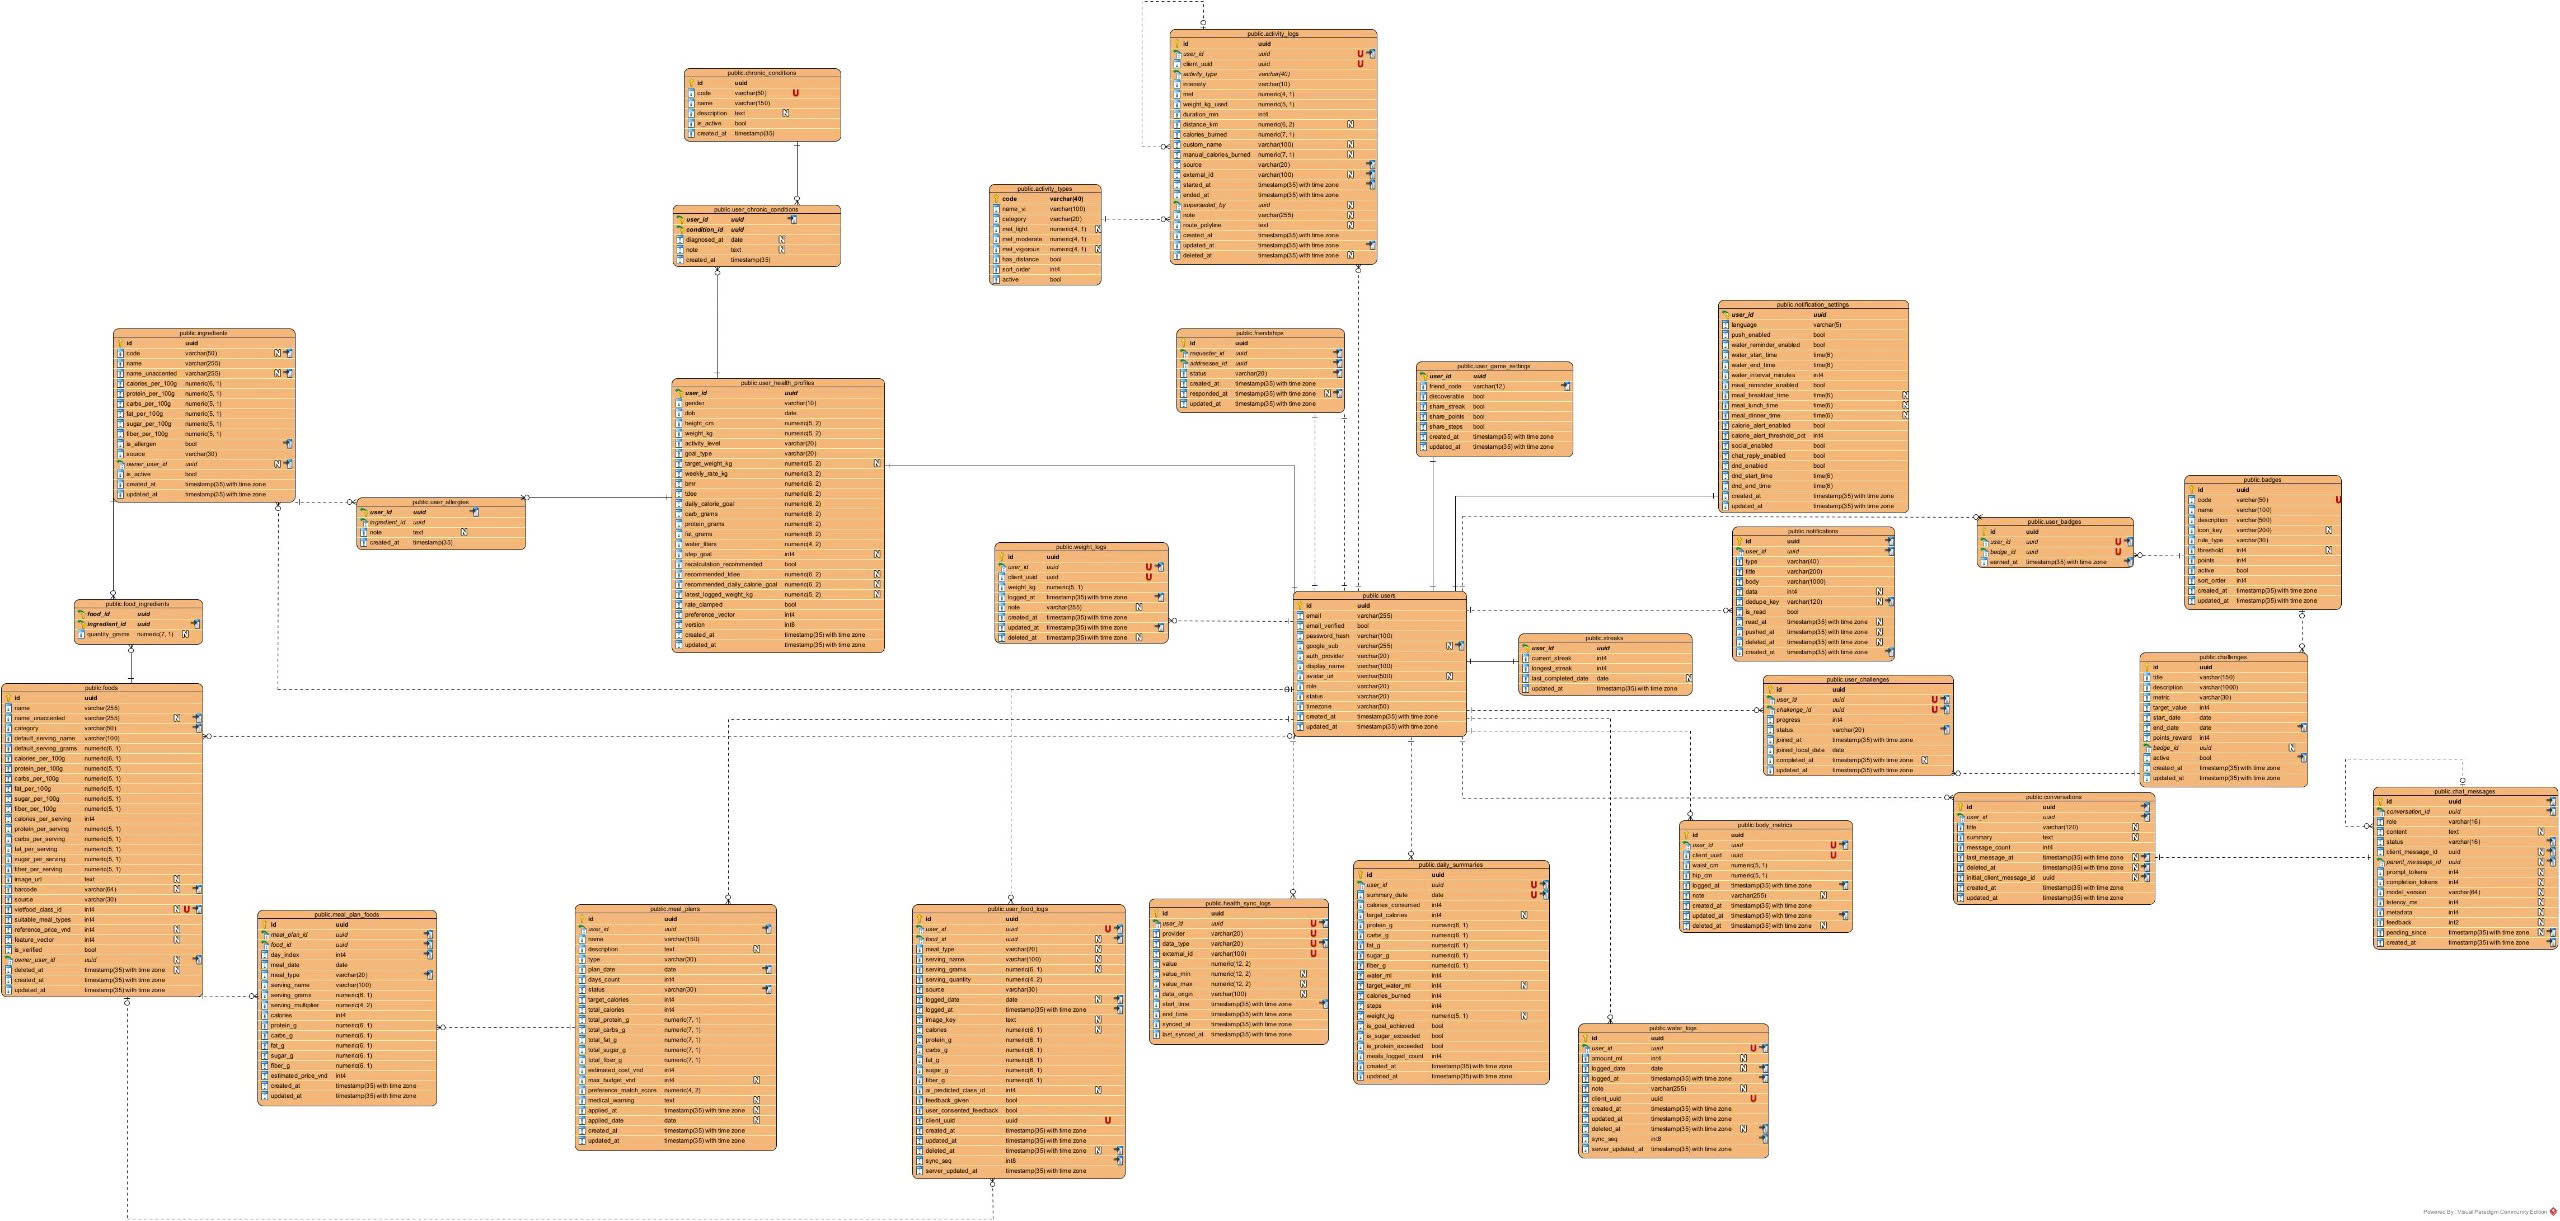
\includegraphics[width=\textwidth]{img/erd.jpg}
    \caption{Sơ đồ cơ sở dữ liệu}
    \label{fig:erd}
\end{figure}

\section{Kết luận chương 2}
\label{sec:2.4}

Trong chương 2, đồ án đã xác định được các actor, UseCase của hệ thống. Từ đó, xây dựng biểu đồ UseCase, kịch bản hoạt động của các UseCase, xây dựng sơ đồ lớp, biểu đồ tuần tự và thiết kế cơ sở dữ liệu.

Trong chương tiếp theo, đồ án sẽ thực hiện cài đặt ứng dụng dựa trên phân tích và thiết kế đã được trình bày trong chương này.



\end{document}